%Alexander Werthmann
\newpage
\usecase{Registrierung}\label{usecse:reg}
\usecasepart{Ausfüllen des Eingabeformulars}
Der User möchte sich registrieren und muss eine Reihe verschiedener Auswahl- und Textfelder mit Daten füllen.

\subsubsection*{Positive Beobachtungen} 
Im linken Bereich auf der Hauptseite des Portals befindet sich der Menüpunkt \emph{ Registrieren}~gut sichtbar zusammen mit einer Reihe anderer Aktionen, wie bereits in obigem Use-Case beschrieben. Das Auffinden dieses Menüpunkts stellt keine Probleme da und der Nutzer kann nach einem Klick auf diesen direkt mit der Registrierung
beginnen.




\problem{Eingabe von Beginn und Ende des Studiums auf den Tag genau}
{Es ist extrem unwahrscheinlich dass ein Alumni der Uni Würzburg noch auf den Tag genau weiß, wann er angefangen oder aufgehört hat zu studieren. Trotzdem befinden sich auf
der Registrierungsseite unter der Überschrift \emph{Ihre Zeit an der Uni Würzburg} zwei Datumseingabefelder \emph{Beginn} und \emph{Ende}, die Eingaben der Form \texttt{dd.mm.yyyy} erwarten.
}
{
Eine Meldung darunter zeigt zwar an, dass man im Falle lückenhafter Erinnerung schätzen solle, allerdings ist es dann fraglich wieso der Tag überhaupt zur Auswahl steht. Die Eingabe eines exakten Datums ist offenbar nicht notwendig für den Seitenbetreiber. Wer allerdings gewissenhaft ein Formular ausfüllen möchte, fühlt sich unwohl bei der Konfrontation mit der eigenen Unwissenheit dieses Datums und noch mehr beim Runden eines vagen Wertes aus dem Gedächtnis. Daher ist diese Eingabe überflüssig und als leichter Fehler der Kategorie 1 zuzuordnen.
}
{Der Tag sollte aus dieser Auswahl komplett gestrichen werden. Da dieses Datum von nahezu jedem Benutzer des Alumni-Portals geschätzt werden wird, liefert er keinen Mehrwert.
} 
\label{prob:reg:wtfday}

\problem{Fehlende Hyperlinks}
{Auf der ersten Registrierungsseite befinden sich zwei Verweise zu Seiten, die nicht, wie allgemein üblich, als Wert eines \texttt{href}-Attributs in Umgebung eines \texttt{\textless a\textgreater}-\texttt{html}-Tags verwendet werden, sondern ohne Hyperlink-Kennzeichnung für den Browser im Fließtext stehen. Das führt dazu, dass der Nutzer den Link erst kopieren und in die URL-Leiste des Browsers kopieren muss, was nicht nur unnötig und nervig ist, sondern zudem auch den professionellen Eindruck der Seite mindert.
}
{Obwohl dieser Fehler im Quellcode vermeidbar und fehlende Links nervig für Nutzer sind, wird jeder verstehen, dass es sich hier um einen Link handelt der in einen Browser eingegeben werden kann. Für große Verwirrung seitens der Anwender sorgt dieses Problem nicht. Es handelt sich um einen mittelschweren Fehler der Kategorie 2.
}
{Dieses Problem ist sehr leicht durch Einsatz eines \texttt{html}-Hy\-per\-links zu lösen.
} 
\label{prob:reg:hyperhyper}

\problem{Überflüssige Date-Picker}
{Die Date-Picker neben den Datumseingaben bei \emph{Geburtstag} auf Seite 1 und bei \emph{Beginn} und \emph{Ende}auf Seite 2 der Registrierung (zu sehen in Abb. \ref{fig:regdatepick}) verführen zur einfachen Eingabe des Datums ohne auf das Format achten zu müssen. Allerdings merkt man schnell, dass diese Freude unbegründet ist, denn es nicht möglich direkt eine Jahreszahl einzugeben. Stattdessen ist der Benutzer gezwungen, Jahr für Jahr zurückzuscrollen was sehr nervig, da langwierig ist (Bsp. Geburtsjahr).
}
{Dem User bleibt überlassen, ob er die Date-Picker nutzt. Es ist aber davon auszugehen, dass er rasch bemerkt, dass er mit gewöhnlicher Eingabe per Tastatur wesentlich schneller voran kommt. Die Date-Picker sind aus diesem Grund leider nicht zu gebrauchen obwohl sie technisch funktionieren. Die Anwesenheit dieser Bedienelemente wirken wiederum negativ auf den Eindruck der Seriosität des Alumni-Portals. Da der Benutzer hier aber noch die Wahl hat das Textfeld durch Tastatureingaben selbst zu befüllen, gehört dieser mittelschweren Fehler in die Problem-Kategorie 2.
}
{Die Date-Picker sollten entfernt werden, da sie in dieser Form definitiv nicht benutzt werden würden und dem Anwender keine Arbeit abnehmen.
}
\label{prob:reg:uselesspickerz}

\begin{figure}
	\centering
		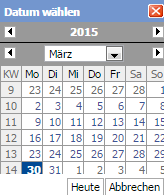
\includegraphics{figures/datepicker.png}
	\caption{Date-Picker für die Datumseingabe}
	\label{fig:regdatepick}
\end{figure}

\problem{Einzelne Buchstaben als Fach auswählbar}
{Unglücklicherweise lassen sich in den Dropdown-Menüs \emph{1. Hauptfach} und \emph{2. Hauptfach} auf Seite 2 der Registrierung, zu sehen in Abb. \ref{fig:regdropdown}, einzelne Buchstaben, die nur als Überschriften dienen sollen, selektieren und somit als Fach auswählen. 
}
{Es handelt sich um einen kleinen Fehler in der Formatierung der Dropdown-Liste, der sofort vom Nutzer erkannt wird. Offensichtlich ist sehr unwahrscheinlich, dass jemand unabsichtlich einen Buchstaben als Fach wählt. Deshalb ist dieser grobe Fehler im \texttt{html}-Code nur mittelschwer und in Kategorie 2 anzusiedeln.
}
{Der Fehler lässt sich leicht beheben indem man zum Beispiel im \texttt{\textless select\textgreater}-Tag das label-Attribut innerhalb eines \texttt{\textless optgroup\textgreater}-Tags setzt. In diesem Fall sollte es bei nicht auswählbaren Elementen wie \glqq A\grqq,\glqq B\grqq~ et cetera verwendet werden.
} 
\label{prob:reg:buchstabe}

\begin{figure}
	\centering
		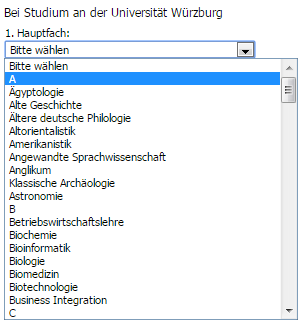
\includegraphics{figures/dropdownlist.png}
	\caption{Dropdown-Liste zur Auswahl des Studienfaches}
	\label{fig:regdropdown}
\end{figure}

\problem{Fehlende Erklärung des roten Sterns \glqq *\grqq}
{Bei vielen Eingabeformularen befindet sich über der oberen rechten Ecke ein roter Stern \glqq *\grqq. Allerdings findet sich nirgends auf der Seite eine Erklärung dieses Zeichens.
Obwohl diese Kennzeichnung heute allgemein für Pflichtfelder benutzt wird, muss berücksichtigt werden, dass die Alumni-Gemeinschaft insbesondere aus älteren Personen besteht, die nicht wissen, wie der Stern zu interpretieren ist. Erst nach einem Klick auf \emph{Weiter} wird der Nutzer darüber informiert, dass er alle mit Stern gekennzeichnete Felder ausfüllen muss.
}
{Besonders deprimierend wird es schließlich für den Nutzer, wenn er ein Pflichtfeld nicht ausfüllt und erst die Eingabefelder suchen muss, die er nicht ausgefüllt hat. Diese werden nicht, wie es in modernen Webseiten üblich ist, hervorgehoben. Dieses schwere Problem sorgt bei unerfahrenen Nutzern für große Verärgerung und ist somit in Kategorie 3 einzustufen.
}
{Eine Möglichkeit zur Verbesserung dieses Problems wäre eine einfache Erklärung des Sternchens anzuzeigen. Wir haben uns im Prototypen allerdings dazu entschlossen die Anzahl der Eingabemasken zu reduzieren und optionale Parameter direkt wegzulassen, sodass eine Kennzeichnen einzelner Formulare nicht mehr notwendig ist.
}

\label{prob:reg:roterStern}
\problem{Unklare oder missverständliche Eingabefelder}
{Leider gibt es auf der Registrierungsseite mehrere Unklarheiten, was in den Formularfeldern eingegeben werden soll. Da sich diese Probleme hinsichtlich der Reaktion
des Nutzers sehr ähnlich sind, sind sie im Folgenden als ein Problem aufgeführt. Dabei bezieht sich \glqq Registrierung(1/2)\grqq ~auf die erste und \glqq Registrierung(2/2)\grqq ~auf die zweite Seite der Registrierung.
\begin{enumerate}
	\item {Registrierung(1/2): \emph{Berufliche Einbindung}: Pop-Up neben \emph{Branche} miss\-ver\-ständ\-lich}
	\item {Registrierung(1/2): Funktion neben dem Email-Eingabefeld wird nicht erklärt}
	\item {Registrierung(2/2): \glqq Abschluss-Auswahl\grqq ~: Ist der bereits erreiche Abschluss oder der aktuelle Abschluss, der in Arbeit ist, gemeint?}
	\item {Registrierung(2/2): \emph{Mitgliedschaft in anderen Vereinen}: Missverständliche Eingabeformulare}	
\end{enumerate}	
Auf der ersten Seite der Registrierung verwirrt das Pop-Up, das sich neben dem \emph{Branche}-Feld befindet. Intuitiv ist nicht sofort klar, dass hier ein eigener
Name für eine Branche eingegeben werden kann.\\
Ebenfalls unerklärt bleibt ein kleines Icon auf beim Email-Eingabefeld, dessen Nutzen sich für Anwender nicht erschließen lässt. Ein neugieriger Anwender erfährt durch einen tapferen Klick auf das Icon, das hier ein Standard-Email-Programm geöffnet wird, dessen Loadscreen (z.B. Microsoft Outlook) dem User den Blick auf die Alumni-Webseite versperrt und ihn so aus seinem aktuellen Umfeld reißt.
Auf Seite zwei der Registrierung befindet sich unter anderem ein Formular, das die Eingabe des \emph{höchsten Abschlusses} fordert. Trotzdem ist diese Formulierung nicht eindeutig,
denn diese könnte zum einen als der höchste erreichte Abschluss oder der Abschluss, der aktuell in Arbeit ist interpretiert werden.\\
Zuletzt fällt ein Textfeld und ein Scrollbalken für die Mitgliedschaft in anderen Vereinen ins Auge. Das Textfeld nimmt sehr viel Platz weg und was hier eingegeben werden soll, ist ebenfalls fraglich, denn unter dem Texteingabefeld bietet eine Dropdown-Liste eine Auswahl an konkreten Vereinen. Diese Darstellung kann ohne weitere Erklärung für redundante Eingaben seitens der Nutzer führen und ist vor allem bei Mehrfachmitgliedschaften sehr problematisch.
}
{Die genannten Probleme lassen sich als missverständliche Eingabefelder zusammenfassen und frustrieren in ihrer Summe Anwender, die selbsterklärende Eingabemasken gewohnt sind. Die aktuelle Darstellung obiger Eingaben verwirrt Benutzer und ist folglich ein schweres Problem (Kategorie 3).
}{
Es sollte bei Eingaben stets der Grundsatz beachtet werden \glqq Wenn du ein Formular erklären kannst, erkläre es. Wenn nicht - Lass es weg!\grqq. Bereits ein kurzer Satz wäre hier schon hilfreich und nimmt dem Nutzer Unsicherheit. Um re\-dun\-dan\-te Eingaben zu vermeiden sollten doppelte Eingabefelder vermieden werden. Man könnte entweder die Dropdown-Liste mit Vorschlägen so erweitern, dass sich eine Menge der wichtigsten/größten Vereine auswählen lässt (für den unwichtigen Rest kann man ein \glqq Andere\grqq-Listenelement einfügen) und das übergroße Textfeld komplett entfernen oder nur eigene Eingaben aus diesem zulassen und die Dropdown-Auswahl entfernen. Da erstere Lösung allerdings das Filtern bei der Suche und Einordnen in eine Datenbank wesentlich erleichtert, ist diese zu bevorzugen.}
\label{prob:reg:unclearinput}


\problem{Verweis auf fehlende Spalte mit Tipps}
{Im Bereich \emph{Zusätzliche Mitgliedschaft} wird darauf hingewiesen, dass ein gewisser Link sich ebenfalls in der \glqq rechten Spalte bei den Tipps\grqq ~befinden würde. Allerdings existieren auf der Seite weder eine rechte Spalte noch Tipps. Die Seite wurde offensichtlich nicht komplett aktualisiert und die Tatsache, dass dem Nutzer auf dieser Seite erste Hoffnung auf Tipps zur Registrierung gemacht werden, dieses Versprechen aber nicht eingehalten wird, ist frustrierend für den Nutzer.
}
{Ein Verweis auf etwas, das nicht mehr aktuell ist, verärgert jeden und zeugt von mangelnder Professionalität der Seitenautoren. Damit wird Kategorie~3 diesem schweren Problem gerecht.
}
{Der Verweis auf die Tipps sollte im aktuellen Zustand der Seite einfach gestrichen werden. Der Link auf den verwiesen wird könnte direkt an dieser Stelle eingefügt werden. Vergleichsweise wurde im Prototyp allerdings eine rechte Spalte eingeführt, die nützliche Tipps zur Registrierung enthält.
} 
\label{prob:reg:missingtipps}

\usecasepart{Abschicken des Eingabeformulars}

Nachdem der Benutzer die Eingabemasken mit allen notwendigen Parametern gefüllt hat, möchte er nun die Registrierung beenden und abschicken. Sobald
er die erste Hälfte der Registrierung beenden will, klickt er auf den \emph{Weiter}-Button und sieht --falls vorhanden-- seine fehlerhaften Eingaben. Hat er nach korrektem
Ausfüllen der ersten Formularseite auch die zweite ausgefüllt und mit einem erneuten Klick auf \emph{Weiter} wieder alle Fehler berichtigt, ist die Registrierung abgeschlossen und wird mit einer Erfolgsmeldung auf der Seite bestätigt.

\problem{Wartezeit nach Registrierung}
{Nachdem die zweite Formularseite mit Daten gefüllt wurde und mit Klick auf den Button \emph{Speichern} bestätigt wurde, erscheint die Meldung \glqq Ihr Freischaltcode, mit dem Sie Ihre persönlichen Login-Daten generieren können, wird Ihnen händisch zugeschickt\grqq. Der User wird zudem zuvor darüber informiert, dass die Überprüfung der Daten Zeit in Anspruch nehmen wird.
}
{Der Anwender ist nun gezwungen zu warten, während seine getätigten Eingaben validiert werden. Da dies verständlicherweise von den Seitenbetreibern ge\-wünscht ist, zum Beispiel um potentiell eingegebene Konto- oder Studiendaten o.Ä. zu überprüfen, ist dies kein Problem (Kategorie 0). 
}
{Eine zukünftige Version des Alumni-Portals könnte den Datenabgleich der Eingaben des Nutzers, wie zum Beispiel \emph{Studienfach}, \emph{Studienzeitpunkt}, da ja ebenfalls ein Name eingegeben wurde, vollautomatisch in der Datenbank der Universität durchführen und dem Nutzer so die Möglichkeit geben, sofort das Alumni-Portal in vollem Umfang zu nutzen.
}
\label{prob:reg:wartezeit}

\problem{Fehlermeldung bei Validierung als Pop-Up realisiert}
{Leider sind alle Fehlermeldungen, die auftreten falls der Nutzer einen ungültigen Wert eingegeben oder ein Pflichtfeld ausgelassen hat, mit einem Aufruf von \texttt{alert()} in Javascript realisiert. Dieser Befehl erzeugt ein kleines Pop-Up, wie in Abb.\ref{fig:regpopup} zu sehen, das Fokus erhält, sodass der Benutzer aus seinem aktuellen Seitenumfeld gerissen wird. Im Pop-Up selbst wird aber nur eine einzelne fehlerhafte Eingabe angezeigt. Wurden mehrere falsche Eingaben getätigt, muss der Nutzer diese einzeln korrigieren und wird nach jeder Korrektur und Klick auf \emph{Weiter} mit einem weiteren Pop-Up belästigt.
}
{Pop-Ups die direkt Fokus erhalten, sind extrem störend für jeden Benutzer, da er gezwungen wird erst das Pop-Up zu schließen, bevor er mit der Browserbedienung fortfahren kann. \texttt{alert()} ist keine geeignete Methode um eine Inputvalidierung durchzuführen. Das aktuelle Design dieses Features ist irreführend und und somit in Kategorie~3 (schweres Problem) einzuordnen.
}
{Moderne Webseiten führen diese Validierungen nicht erst beim Absenden des Formulars, sondern direkt während der Eingabe aus. Eine interaktive Fehleranzeige erfreut Anwender, die ihre Fehler sofort berichtigen können ohne in ihrem weiteren Vorgehen unterbrochen zu werden. Der Prototyp enthält eine solche interaktive Validierung, die sogar die Datenbank über eine bereits vergebene Mailadresse informiert.}
\begin{figure}
	\centering
		
\includegraphics{figures/regpopup.png}
	\caption{Pop-Up bei falschen Eingaben}
	\label{fig:regpopup}
\end{figure}

\label{prob:reg:popup}
\problem{Bereits vergebene Mail resultiert in Neuladen der Seite}
{Ein weiteres, störendes Problem auf der Registrierungsseite ist deren Reaktion darauf, dass ein User eine bereits verwendete E-Mail-Adresse benutzen will. Zwar wird dies von der Webseite bemerkt und es wird (mit einem Pop-Up) darauf hingewiesen, allerdings lädt sich die Seite dabei neu und etwa die Hälfte aller Eingabemasken werden durch diesen Vorgang geleert. Die Daten dieser Eingabefelder, die der Nutzer bereits eingetragen hat, müssen dadurch erneut eingegeben werden.
}
{Ein Anwender der erst alle vorgeschlagene Eingabefelder ausfüllt und dann die Hälfte der Informationen nochmals eingeben muss, ist frustriert und wird, falls dies mehrmals passiert, definitiv auf eine Registrierung verzichten. Dieses Problem ist schwerwiegend und deshalb Kategorie~3 zuzuordnen.
}
{Die Überprüfung auf eine bereits vorhandene E-Mail-Adresse sollte optimalerweise direkt bei der Eingabe erkannt und gemeldet werden. Ein schlankes Backend erledigt diesen Lookup-Vorgang on-the-fly ohne viel Ressourcen zu verbrauchen. Der Prototyp enthält ein solches Feature und meldet den Fehler ohne Pop-Up, dafür aber mit farbiger Fehlermarkierung.
}  
\label{prob:reg:vergivenmail}


\problem{Fehlende/falsche reguläre Ausdrücke bei Formularvalidierung}
{Das gravierendste Problem auf der Registrierungsseite ist allerdings, dass bei mehreren Eingabefeldern keine korrekten regulären Ausdrücke zur Validierung verwendet wurden. Es ist etwa möglich eine reine Buchstabensequenz als Postleitzahl einzugeben, oder was noch schlimmer ist eine ungültige E-Mail-Adresse, wie zum Beispiel ein einfaches \glqq \texttt{@}\grqq.
}
{Eine fehlerhafte E-Mail-Adresse führt dazu, dass der Nutzer womöglich endlos auf eine Freischaltung wartet und den Fehler nie bemerkt. Er kann die Seite durch diesen Umstand also gar nicht mehr benutzen. Die falschen regulären Ausdrücke sind ein fataler Fehler und damit eindeutig als Kategorie~4-Problem einzustufen.}
{Das Problem kann einfach gelöst werden, indem korrekte reguläre Ausdrücke zur Validierung benutzt werden.
} 
\label{prob:reg:regex}

